
\documentclass{article}
\usepackage{geometry}
\usepackage[utf8]{inputenc}

\usepackage{fancyhdr}
\pagestyle{fancy}
\hoffset=0.3in
\voffset=-0.2in
\headsep=0.5in
\lhead{}
\chead{}
\rhead{\thepage}
\lfoot{}
\cfoot{}
\rfoot{}
\renewcommand{\headrulewidth}{0pt}
\renewcommand{\footrulewidth}{0pt}
\setlength{\parindent}{4em}
\paperheight=11in
\textheight=9.0in
\usepackage[pdftex]{graphicx}
\large

\usepackage{titlesec}
\titleformat*{\section}{\LARGE}
\titleformat*{\subsection}{\Large}
\titleformat*{\subsubsection}{\Large}

\usepackage{alltt}

%\usepackage{tocloft}

%\renewcommand\cftsecfont{\normalfont}
%\renewcommand\cftsecpagefont{\normalfont}
%\renewcommand{\cftsecleader}{\cftdotfill{\cftsecdotsep}}
%\renewcommand\cftsecdotsep{\cftdot}
%\renewcommand\cftsubsecdotsep{\cftdot}
%\renewcommand\cftsubsubsecdotsep{\cftdot}

%\usepackage{fullpage}
%\usepackage{setspace}
%\doublespacing
\linespread{2}
\usepackage{setspace}
\usepackage{cite}


% declare the path(s) where your graphic files are
\graphicspath{{./images/}}
 % and their extensions so you won't have to specify these with
 % every instance of \includegraphics
 \DeclareGraphicsExtensions{.pdf,.jpeg,.png}
%\usepackage{fancyhdr}

\usepackage{threeparttable}

\usepackage{enumerate}

%\usepackage{tgbonum}
%\usepackage{ascii}
%\usepackage[T1]{fontenc}
\renewcommand*\contentsname{\empty}
\renewcommand{\listtablename}{\empty}
\renewcommand{\listfigurename}{\empty}
%\renewcommand{\thebibliography}{\empty}
\renewcommand\refname{}



\begin{document}

\begin{titlepage}
\begin{center}
	\begin{Large}
	\textbf{Integrating Pattern Matching Within String Scanning}\\
	\end{Large}
	\begin{large}
	\vspace{5 pc}
	A Thesis\\
	Presented in Partial Fulfillment of the Requirements for the\\
	Degree of Master of Science\\
	with a\\
	Major in Computer Science\\
	in the\\
	College of Graduate Studies\\
	University of Idaho\\
	by\\John H. Goettsche\\
	\vspace{5 pc}
	Major Professor: Clinton Jeffery, Ph.D.\\
	Committee Members: Robert Heckendorn, Ph.D.; Robert Rinker, 	Ph.D.\\
	Department Administrator: Gregory Donohoe, Ph.D.\\
	\vspace{8 pc}
	June, 2015
	\end{large}
	\end{center}
\end{titlepage}

	%\fontfamily{lmss}
	%\selectfont 
	
\thispagestyle{empty}

\pagebreak
\large
\thispagestyle{fancy}
\pagenumbering{roman}
\addcontentsline{toc}{section}{Authorization to Submit Thesis}
\begin{center}
\textbf{Authorization to Submit Thesis}
\end{center}
This Thesis of John H. Goettsche, submitted for the degree of Master of Science with a Major in Computer Science and titled ``Integrating Pattern Matching Within String Scanning,'' has been reviewed in final form.  Permission, as indicated by the signatures and dates below, is now granted to submit final copies to the College of Graduate Studies for approval.\\
\vspace{0.3in}
\begin{singlespace}
\noindent
	Major Professor:\hspace{0.8in}\makebox[2.5in]{\hrulefill} Date: \makebox[1.0in]{\hrulefill} \\
	\-\hspace{2.0in}Clinton Jeffery, Ph.D.\\
	\vspace{0.1in}\\
	Committee Members:\hspace{0.5in}\makebox[2.5in]{\hrulefill} Date: \makebox[1.0in]{\hrulefill} \\
	\-\hspace{2.0in}Robert Heckendorn, Ph.D.\\
	\vspace{0.1in}\\
	\-\hspace{2.0in}\makebox[2.5in]{\hrulefill} Date: \makebox[1.0in]{\hrulefill} \\
	\-\hspace{2.0in}Robert Rinker, Ph.D.\\
	\vspace{0.1in}\\
	Department Administrator: \makebox[2.5in]{\hrulefill} Date: \makebox[1.0in]{\hrulefill} \\
	\-\hspace{2.0in}Gregory Donohoe, Ph.D.\\
\end{singlespace}

\pagebreak

\addcontentsline{toc}{section}{Abstract}
\begin{center}
\textbf{Abstract}
\end{center}

A SNOBOL4 like pattern data type and pattern matching operation were introduced to the Unicon language in 2005, but patterns were not integrated with the Unicon string scanning control structure and hence, the SNOBOL style patterns were not adopted as part of the language at that time.  The goal of this project is to make the pattern data type accessible to the Unicon string scanning control structure and vice versa; and also make the pattern operators and functions lexically consistent with Unicon.  To accomplish these goals, a Unicon string matching operator was changed to allow the execution of a pattern match in the anchored mode, pattern matching unevaluated expressions were revised to handle complex string scanning functions, and the pattern matching lexemes were revised to be more consistent with the Unicon language.

\pagebreak

\addcontentsline{toc}{section}{Acknowledgements}
\begin{center}
\textbf{Acknowledgements}
\end{center}
I would like to acknowledge my major professor Clinton Jeffery who guided my research on this project.  I would also like to acknowledge the Special Information Services department of the National Library of Medicine for the financial support that made my research possible.

\pagebreak

\addcontentsline{toc}{section}{Dedication}
\begin{center}
\textbf{Dedication}
\end{center}
To all my fellow Land Surveyors who have searched for or sought to develop software that is used the way surveyors actually work. 

\pagebreak
\linespread{1}
\begin{center}
\textbf{Table of Contents}
\end{center}
\addcontentsline{toc}{section}{Table of Contents}
\tableofcontents

\pagebreak
\begin{center}
\textbf{List of Tables}
\end{center}
\addcontentsline{lot}{section}{List of Tables}
\listoftables
	
\pagebreak
\begin{center}
\textbf{List of Figures}
\end{center}
\addcontentsline{lof}{section}{List of Figures}
\listoffigures

\pagebreak

\pagenumbering{arabic}
\textbf{\section{Introduction}}
Many different string scanning and pattern matching systems have been developed in order to enhance programmers' productivity in analyzing strings.  Modern high level languages tend to offer regular expressions and context free grammars for their string processing.  Analysis of strings often requires functionality beyond what these classes of languages offer.  SNOBOL4 was the most successful of the early string processing languages\cite{Snobol, Gaikaiwari2005}.  A pattern data type was employed in SNOBOL4 along with pattern operators and functions to perform the analysis.

Icon is a successor to SNOBOL4, which expanded upon the goal directed evaluation with generators and backtracking that was implicit in SNOBOL4's pattern matching\cite{GriswoldIcon, Gaikaiwari2005}.  It uses a string scanning control structure that passes through the subject string with a set of commands to manipulate and analyze its contents.  When Unicon was developed, its core elements came directly from Icon, including its string scanning facilities\cite{JefferyUnicon}. Many of the Icon string scanning functions resemble SNOBOL4 patterns, but they are different in both how they are processed as well as their functionality.  Many Icon programmers have expressed a desire for the functionality of SNOBOL4 patterns\cite{Griswold1980}.

While SNOBOL patterns are instances of a structured data type that are used deductively to test whether the pattern exists within a subject string, a string scanning environment uses a set of functions to inductively analyze or extract data from the subject string.  Patterns are pre-defined and applied later, while string scanning is performed as string scanning functions are executed.  Patterns allow composition and re-use in more flexible ways than is the case for code, which only has procedure and co-expression granularity.  A co-expression is an independent, encapsulated thread-like context, allowing the results of an expression to be retrieved one at a time\cite{JefferyUnicon}.

This paper briefly explores the background of SNOBOL4 patterns and Unicon string scanning functions.  It discusses design considerations for integrating SNOBOL4 patterns within Unicon string scanning environments, a description of how proposed changes were implemented, and the benchmarks used to evaluate the success of the integration.

\pagebreak
\textbf{\section{Background}}
SNOBOL was developed by David Farber, Ralph Griswold and Ivan Polonsky at Bell Telephone Laboratories in 1962.  SNOBOL4 was developed in 1967 and had many of the features that are included in popular dynamic programming languages including dynamic typing, eval and garbage collection.  Its pattern data type was its most important contribution to string processing.  Patterns could be as simple as a single character or a set of characters in a particular order, or they could be a complex arrangement with alternative character sets and pattern functions.  The pattern data type enabled the user to define and store patterns in variables to be used later when they were desired\cite{Snobol}.  

\textbf{\subsection{Icon and Unicon}}
One of the developers of SNOBOL4, Ralph Griswold, joined the faculty of the University of Arizona and developed the Icon programming language which was more readable and simpler to use than SNOBOL\cite{JefferyUnicon}.  Griswold used his experience with SNOBOL4's generators and backtracking in its pattern matching to develop goal directed evaluation\cite{Gaikaiwari2005}.  SNOBOL4 patterns were not incorporated in Icon.  Instead Griswold developed an extensive string scanning system where a variety of functions and operations are executed in order to analyze and extract information from a subject string as the cursor location advances.  Unlike most other languages, Icon considers the string as a primitive data type in its own right, rather than an array of characters\cite{GriswoldIcon}.  

Using the same Icon source code, Unicon was developed to include modern software features such as objects, networks and databases\cite{JefferyUnicon}.  The string scanning control structure of Icon is a part of the Unicon programming language, yet the desire of researchers and developers for SNOBOL4's pattern data type and pattern matching facilities has persisted.  Sudarshan Gaikaiwari adopted SNOBOL4 patterns to the Unicon language for his master's thesis in 2005.  In his thesis, he added the pattern data type, and provided pattern matching functions and operators to execute the pattern searches\cite{Gaikaiwari2005}.  The pattern data type was kept separate from the string scanning control structure, which may not execute pattern matching operations.  This thesis refines Gaikaiwari's work to be more naturally incorporated in the Unicon language, allowing string scanning environments to utilize the pattern matching functionality and vice-versa.

\textbf{\subsection{Pattern Matching}}
The purpose of pattern matching is to determine the presence of a predefined pattern within a subject string.  The pattern matching operation is initialized in Unicon by using the \texttt{??} operator \cite{Gaikaiwari2005}.  The following expression results in the \texttt{subject} having a pattern match performed with \texttt{pattern}:\\
\begin{alltt}
        subject ?? pattern
\end{alltt}
If the pattern is found in \texttt{subject} then the expression succeeds and the first substring matching the pattern is returned; otherwise it fails.

A pattern is constructed by assigning it to a series of simple pattern components and pattern operators, alternation \texttt{.|} and concatenation \texttt{||}.  An alternation operation succeeds if either of the patterns on either side of the operator is found.  A concatenation operation succeeds if the pattern on the left is immediately followed by the pattern on the right.

For example, if the user wanted to define a pattern called \texttt{"pat"} that identifies whether \texttt{"bean"} or \texttt{"been"} as in a subject string.  The follow code would produce that result:\\
\begin{alltt}
        pat := "be" || ( "a" .| "e" ) || "n"
\end{alltt}
The figure below illustrates the pattern definition.
\begin{figure}[ht!]
\centering
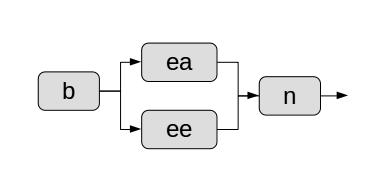
\includegraphics[width=90mm]{bean.jpg}
\caption{Pattern Example\label{overflow}}
\end{figure}
when the pattern match is performed on a subject string, it will first search for \texttt{"be"}.  When it finds \texttt{"be"}, it will then check to see if it is followed by an \texttt{"a"}.  If it fails it will backtrack to the successful \texttt{"be"} and check to see if it is followed by \texttt{"e"}.  If it fails again, it will backtrack again.  There not being another option, it will backtrack again past the \texttt{"be"} and will search for another \texttt{"be"} and do the process again until it succeeds at each of the three parts of the pattern. 

Consider the string \texttt{"I've been there!"}. The pattern will iterate through each of the letters until it reaches the \texttt{"be"}.  Then it will not match \texttt{"a"} and then try \texttt{"e"} where it succeeds.  Then it will check for an \texttt{"n"}.  The check succeeds at the end of the pattern and will suspend \texttt{"been"}. 

\pagebreak
\textbf{\section{Design Considerations}}
To integrate pattern matching with Unicon string scanning required consideration of how a user would execute a pattern match in the string scanning environment and string scanning functions in the pattern matching operation.  The following questions had to be addressed.  What parameters are necessary for their execution?  From what environment are they being called?  How are they going to be utilized and under what conditions for each implementation?  Also, the pattern functions and operators will have to be consistent lexically and functionally with the Unicon language.

\textbf{\subsection{Pattern matching statements}}
SNOBOL pattern matching can be executed in either anchored or non-anchored mode.  The anchored mode requires the match to start on the first character of the subject string while in the non-anchored mode the match can start at any location in the subject string\cite{Snobol}.  The pattern matching operation adapted by Gaikaiwari operates in the non-anchored mode\cite{Gaikaiwari2005}.  Gaikaiwari's pattern matches only produce one value at a time, but since they suspend instead of return that value, the cursor position is stored so the next pattern can be applied to the remainder of the string to produce the next value\cite{JefferyUnicon}.

The pattern matching statements in SNOBOL4 and Gaikaiwari's Unicon implementation are in the following form:\\

\begin{table}[ht]
	\centering
	\begin{tabular}{c c}
		SNOBOL4 & Gaikaiwari's Unicon \\
		\texttt{ SUBJECT  PATTERN }& 
		
		\texttt{ subject ?? pattern }

	\end{tabular}
\end{table}
\noindent
In both examples, the subject is scanned to see if it contains the pattern.  If it succeeds, then a substring of the subject that fits the pattern is produced.  Gaikaiwari's syntax starts the pattern matching operation with the use of the \texttt{??} operator while in SNOBOL4 the operation is implicit with the subject followed by the pattern.  Since the Unicon string scanning operator is \texttt{?} and used in the following syntax:\\

\begin{alltt}
   subject ? expr
\end{alltt}

Gaikaiwari's operator is intended to match Unicon lexically and syntactically, and its explicit form is arguably easier to read than separating the subject and pattern with white space.   

To integrate pattern matching into the Unicon language, it is necessary to consider which mode is appropriate for the current environment.  If it is being executed outside of a Unicon string scanning environment, the cursor position or index of the string has not been established.  Therefore the non-anchored mode is appropriate for basic pattern matching operations.  This allows a pattern to be matched anywhere within the subject string.  

In the anchored mode the pattern match begins at the current cursor or index location.  If the pattern fails at the first character then the entire pattern will fail to match and will not look for an alternate match later in the subject string.  Sometimes the user wishes to start the pattern match at the first location in the subject string, as though it was in the anchored mode.  In these situations, defining the pattern with a first element of \texttt{Pos(1)} has the desired effect.

\textbf{\subsubsection{Pattern matching within String Scanning}}
In the Unicon string scanning environment the functions operate in relation to the cursor position of the subject string.  It is an inductive process where the data is analysed by executing a series of functions on the subject string.  The cursor location or index is adjusted depending on the success or failure of each expression.  When executing pattern matching from within a Unicon string scanning environment, the cursor or index location is established.  Therefore, in order to maintain this indexing process in the string scanning environment, pattern matching executes in the anchored mode.  

Unicon's \texttt{?} operator sets the cursor location to the first position in the subject string and then the scanning expression, usually a block expression containing a series of calls to scanning functions, is executed.  Scanning functions \texttt{move()} and \texttt{tab()} as well as the unary operator \texttt{=}, move the cursor upon success. For this reason anchored mode was introduced by extending the unary \texttt{=} operator.  Given a pattern operand, \texttt{=p} om the anchored mode, with the cursor being advanced to the end of the match if there is success.  If the user wishes the pattern to be found at the end of the subject string.  In these situations, defining the pattern with a final element of \texttt{Pos(0)} has the desired effect.

\textbf{\subsubsection{String Scanning within Patterns}}
Patterns are pre-defined and are used deductively to search a subject string for the pattern.  A regular pattern match is performed in the un-anchored mode and establishes the cursor locations for the beginning and end of a pattern when it is found.  This is done by iterating through the subject string until a match is found.  It is possible for a string scanning function to be performed as the pattern matching process iterates through the cursor or index locations.

Gaikaiwari's pattern matching facilities allow simple single depth function calls to be made with an \textit{unevaluated expression} enclosed in backquotes.  His unevaluated expressions can handle procedure calls such as \texttt{`foo(2 , "bar")`} but can not handle nested function calls like \texttt{tab(upto(somecset))}\cite{Gaikaiwari2005}.  Therefore the unevaluated expressions implementation needed to be revised to handle more complex functions calls which are common when performing string scanning operations.

\textbf{\subsection{SNOBOL4 and Unicon pattern operators}}
The pattern operators for Unicon were defined by Gaikaiwari in his Master's Thesis.  Although they are lexically different, they are functionally identical to SNOBOL4 pattern operators.  The pattern concatenation operator is similar to the string concatenation operator in that it has the end result of the first pattern or string being followed by the second pattern or string.  But, they differ in that string concatenation joins two strings, while pattern concatenation constructs a pattern that, when applied, finds a match for the first pattern in the subject string that is followed by the second pattern.

The Unicon operator for string concatenation was modified to recognize whether the expression contains a pattern.  Since Gaikaiwari's pattern concatenation and Unicon's string concatenation operators did not have the same order of precedence, the assignment operators' order of precedence was adjusted to maintain their semantics.  

Intermediate assignment \texttt{=>}, conditional assignment \texttt{->} and cursor assignment \texttt{.>} were changed lexically to use the \texttt{>} symbol in the right position of the lexeme to represent an assignment within patterns.  This makes them more consistent lexically.  The SNOBOL4 lexemes appear almost random in their selection and Gaikaiwari's also lacked consistency. The Immediate Assignment, Conditional Assignment and Cursor assignment are \texttt{=>}, \texttt{->} and \texttt{.>} respectively.\\

\begin{table}[ht]
	\caption{Pattern Operators}
	\centering
	\begin{tabular}{|l|l|l|l|}
		\hline\hline
		Operation & SNOBOL4 & Gaikaiwari & New\\
		\hline
		Concatenation & $<<$implicit$>>$ & \&\& & $||$ \\
		Alternation & $|$ & $.|$ & $.|$ \\
		\hline
		Immediate Assignment & \$ & \$\$ & \texttt{=>} \\
		Conditional Assignment & . & \texttt{->} & \texttt{->}\\
		Cursor Assignment & @ & .\$ & \texttt{.>} \\
		\hline
		Unevaluated Expression & $*$x & `x` & `x` \\
		\hline
	\end{tabular}
\end{table}

\vspace{1 pc}
\textbf{\subsection{SNOBOL4 and Unicon pattern functions}}
Since the demand for SNOBOL4 patterns to be added to Unicon is coming from SNOBOL4 users, it is important that the Unicon pattern functions appear as similar to SNOBOL4 pattern functions as possible, while being lexically consistent with Unicon.  Gaikaiwari's pattern functions 
are functionally the same as SNOBOL4 patterns, but appear somewhat disconnected from Unicon lexically.  The way in which Unicon handles its csets and strings makes some functions redundant or inconsistent with Unicon, therefore some of the pattern functions will be removed. 

Table 2 shows the SNOBOL4 primitive functions and the new Unicon pattern functions.  In most cases, the function is lexically similar to SNOBOL4 with the first character being capitalized and the following letters in lower-case, with exceptions for FAIL and ABORT.  Other changes are described in the example uses of the functions below: \\

\begin{table}[ht]
	\centering
	\caption{Pattern Functions}
	\begin{threeparttable}
		\centering
		\begin{tabular}{|l|l|l|}
			\hline\hline
			SNOBOL4 & Gaikaiwari & New \\
			\hline
			ABORT & PAbort() & Cancel() \\
			ANY(c) & PAny(c) & Any(c)* \\
			ARB & PArb() & Arb() \\
			ARBNO(p) & PArbno(p) & Arbno(p) \\
			BAL & PBal() & Bal() \\
			BREAK(c) & PBreak(c) & Break(c) \\
			FAIL & PFail() & Fail() \\
			FENCE & PFence() & Fence() \\
			LEN(n) & PLen(n) & Len(n) \\
			NOTANY(c) & PNotAny(c) & * \\
			POS(n) & PPos(n) & Pos(n)** \\
			REM & PRest() & Rem() \\
			RPOS(n) & PRpos(n) & ** \\
			RTAB(n) & PRtab(n) & ** \\
			SPAN(c) & PSpan(c) & Span(c)  \\
			TAB(n) & PTab(n) & Tab(n)** \\
			\hline
		\end{tabular}
		
		\begin{tablenotes}
      		\small
      		\item * see 3.3.1 complements with functions
      		\item ** see 3.3.2 index related functions
      	\end{tablenotes}
	\end{threeparttable}
\end{table}

\vspace{1 pc}
\textbf{\subsubsection{Complements with functions}}
The complement operator allows the user to get the complement of a given cset, or a cset containing all the characters not included in the given cset.  Therefore the functionality of the \texttt{NotAny(c)} function can be achieved by using the complement operator with a cset in the \texttt{Any} function as \texttt{Any($\sim$c)}.  The run time for each method is the same on average.

\vspace{1 pc}
\textbf{\subsubsection{Index Related Functions}}
The \texttt{POS(n)}, \texttt{RPOS(n)}, \texttt{TAB(n)} and \texttt{RTAB(n)} SNOBOL4 functions all work directly with the cursor location or index.  In Unicon the index value is the number of spaces to the right from the left end of string with the first position being 1 or starting at the right end of the string starting with zero and subtracting the number of spaces to the right end of the string\cite{JefferyUnicon}.   The illustration below demonstrates the Unicon cursor position values for the string \texttt{"Unicon"} with the vertical bars representing the index locations:\\

\begin{alltt}
                   -6  -5  -4  -3  -2  -1  0
                   | U | n | i | c | o | n |
                   1   2   3   4   5   6   7
\end{alltt}

The SNOBOL4 cursor locations for the \texttt{RPOS(n)} and \texttt{RTAB(n)} functions the cursor locations are as follows:\\

\begin{alltt}
   RPOS(n) & RTAB(n)    6   5   4   3   2   1   0
                        | S | N | O | B | O | L |
   POS(n) & TAB(n)      1   2   3   4   5   6   7
\end{alltt}

Integration of the SNOBOL4 \texttt{RPOS(n)} and \texttt{RTAB(n)} functions with the Unicon string indexes can be achieved with \texttt{Pos(-n)} and \texttt{Tab(-n)} functions, making \texttt{RPOS(n)} and \texttt{RTAB(n)} redundant.

\pagebreak
\textbf{\section{Implementation}}
Figure 2 shows the relationship of the Unicon tools for translation, compiling and execution of a Unicon program.  The front-end compiler, called unicon,  translates the unicon code into icon code\cite{JefferyImp}.  This is where the pattern definitions and their component parts are identified and converted to their respective pattern function calls for the runtime system\cite{JefferyImp}.  The function lists are generated for the unevaluated expressions.  Icont compiles Icon code down to virtual machine code\cite{JefferyImp}.  Iconx is the Icon and Unicon virtual machine\cite{JefferyImp}, where the \texttt{pattern\_match()}, \texttt{ResolveReferences} and \texttt{ResolveList} functions are executed. 

\begin{figure}[ht!]
\centering
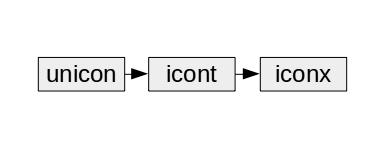
\includegraphics[width=90mm]{compiler.jpg}
\caption{Unicon tools organization\label{overflow}}
\end{figure}


To implement the integration of patterns and string scanning, the following changes to the Unicon language had to be made:
\begin{itemize}
\item Modify Unicon's runtime to execute pattern matching in the anchored mode when a pattern operand is used with the tabmat operator in a string scanning environment.
\item Modify the unevaluated expression operand in the pattern matching operation to handle nested function calls within  parameters, as used in string scanning function calls.
\item Modify patterns to work off of the \texttt{\&subject} and \texttt{\&pos} keywords.
\item Modify the pattern source files to address the functional changes for \texttt{Pos(n)} and \texttt{Tab(n)}.
\item Modify function definitions for the Unicon build.
\item Modify the concatenation operator to function with patterns.
\end{itemize}

\textbf{\subsection{Pattern matching statements}}
The pattern matching operation \texttt{\&\&} in Gaikaiwari's 2005 Master's thesis was performed in the non-anchored mode.  The anchored pattern matching operation was defined in the pattern C library code as a part of the \texttt{internal\_match} operation, but the \texttt{Anchored\_Mode} identifier was set to false.  The default location of the index was set to 1.  The arguments for the \texttt{internal match} operation were changed to include both the mode and cursor location.  This allows the \texttt{internal\_match} to be called and initiated from any location of the subject string.

\textbf{\subsubsection{Anchored mode from string scanning}}
Integrating the pattern matching system into the Unicon string scanning environment requires that the pattern matching be performed in the anchored mode, since the string scanning functions operate from the index or cursor position.  As described in section 3.1.1 \textsl{Pattern matching within String Scanning}, the unary operator \texttt{=} was determined to be an ideal choice for initiating a pattern match in a string scanning environment.  The use of an equals \texttt{=} before a pattern variable triggers the anchored mode pattern matching operation.\\
 
\begin{alltt}
   subjectString ? {
      match := =pattern
   }
\end{alltt}

The tabmat operator was modified to accept operands of type pattern.  In the event that a pattern is its argument, tabmat initiates a pattern match in the anchored mode, otherwise it functions normally.  This section of RTL (Run Time Language) \cite{walker1994} code from omisc.r in Unicon's runtime system identifies whether the argument is a pattern or a string and assigns its return value, and performs the assignments required for the pattern match.

\begin{alltt}
operator\{*\} = tabmat(x)
   if is:pattern(x) then \{
      abstract \{
         return string
         \}
      body \{
         int oldpos, start, stop, subject_len, new_len;
         struct b_pattern *pattern = NULL;
         tended struct b_pelem *phead = NULL; 
         char * pattern_subject;
         CURTSTATE();
         
         /*
          * set cursor position, and subject to match
          */
         oldpos = k_pos;
         pattern_subject = StrLoc(k_subject);
         subject_len = StrLen(k_subject);
         pattern = (struct b_pattern *)BlkD(x, Pattern);
         phead = (struct b_pelem *)ResolvePattern(pattern);
         
         /*
          * runs a pattern match in the Anchored Mode and returns
          * a sub-string if it succeeds.
          */
         if (internal_match(pattern_subject, subject_len, 
               pattern->stck_size, phead, &start, &stop, 
               k_pos - 1, 1))\{
            /*
             * Set new &pos.
             */ 
            k_pos = stop + 1;
            EVVal(k_pos, E_Spos);	
            oldpos = k_pos;
         
            /*
             * Suspend sub-string that matches pattern.
             */
            suspend string(stop - start, StrLoc(k_subject)+ start);
            pattern_subject = StrLoc(k_subject);
            if (subject_len != StrLen(k_subject)) \{
               k_pos += StrLen(k_subject) - subject_len;
               subject_len = StrLen(k_subject);
               \}
            \}
            
         /*
          * If tab is resumed, restore the old position and fail.
          */
         if (oldpos > StrLen(k_subject) + 1)\{
            runerr(205, kywd_pos);
            \} 
         else \{
            k_pos = oldpos;
            EVVal(k_pos, E_Spos);
            \}
         fail;
         \}
      \}
\end{alltt}

As shown above, the tabmat operator checks to see if the parameter is a pattern.  If a pattern is found, \texttt{CURTSTATE()} is called.  Then \texttt{k\_pos} and \texttt{k\_subject} are assigned \texttt{\&pos} and \texttt{\&subject} respectively.  The \texttt{internal\_match()} function is called in the anchored mode.  The index or cursor location is passed along to begin the pattern match where the string scanning had left off.  Finally, if the pattern was successful, then it would have to suspend the matching pattern and update the index or cursor location.  If it failed then it would revert to the previous index or cursor location.  

\textbf{\subsubsection{String Scanning Functions as Unevaluated Expressions}}
In Gaikaiwari's implementation of patterns, functions can be called in a pattern using the unevaluated expression notation by placing the function call in back quotes, for example: \texttt{pattern := `tab(3)`}.  This allows the user to place simple Unicon string scanning function calls and procedure calls in the pattern definition, but only if \texttt{tab(3)} impacts subsequent pattern match operations.

The first phase of the analysis of an unevaluated expression occurs during compile time.  In this process, the \texttt{process\_uneval()} procedure in \texttt{tree.icn}, calls the \texttt{emit\_code\_for\_uneval()} procedure which generates a list to be interpreted during runtime.  Both of these procedures are found in the tree.icn file of the Unicon implementation.\\
\begin{verbatim}
procedure emit_code_for_uneval(funcname)
   L := []
   tab(many('`'))
   temp := tab(upto('(.')) 
   if \temp == "\\" then temp := "\\\\"
   put(L,\temp)
   while tab(upto(&letters)) do {
      temp := tab(many(&letters))
      put(L,temp)
      }
   writes(yyout,funcname, "(")
   writes(yyout, "[")
   every temp := !L\ (*L -1) do {
      writes(yyout, "\"", temp,"\",")
      }
   writes(yyout, "\"", L[*L], "\"")
   writes(yyout, "])")
   return
end
\end{verbatim}
The list generated in this process is similar to LISP in that the first element is the function to be called and the remaining elements are the parameters.  Unfortunately, Gaikaiwari's implementation could not handle functions or procedure calls as parameters within another function or procedure call as is common with some string scanning functions.  For example \texttt{tab(upto('e'))}, the \texttt{tab()} function requires an integer value which is acquired by the \texttt{upto()} function that scans a string until it reaches an 'e' character.  Gaikaiwari's procedure would generate a list \texttt{["tab", "upto", "e"]}, where \texttt{upto} would not be a function call, but instead treated as a string.  This procedure had to be revised to handle function calls as parameters in a function call.  To navigate nested function calls, a recursive procedure generates the list for each function that is used as a parameter in the parent function.  It was implemented with the following procedures: \\
\begin{verbatim}
global list_of_invocables

procedure writes_code_for_uneval(L)
local i
   writes(yyout, "[")
   every temp := L[i := 1 to *L] do {
      if type(temp) == "list" then {
         writes_code_for_uneval(temp)
         } 
      else {
         writes(yyout, image(temp))
         if i = 1 then {
            /list_of_invocables := []
            put(list_of_invocables, temp)
            }
         if i < *L then {
            writes(yyout, ", ")	
            }
         }
      }
   writes(yyout, "]")
   return
end

procedure make_list_for_uneval(L, word)
   while tab(upto(word)) do {
      temp := tab(many(word))
      if proc(temp) | move(1) === "." then {
         L1 := []
         put(L1, temp)
         L1 := make_list_for_uneval(L1, word)
         put(L, L1)
         }
      else {
         put(L, temp)
         }
      }
   return L
end

procedure emit_code_for_uneval(funcname)
   L := []
   tab(many('`'))
   temp := tab(upto('(.')) 
   if \temp == "\\" then temp := "\\\\"
   put(L, \temp)
   word := &letters ++ &digits ++ '\'\"&~'
   L := make_list_for_uneval(L, word)
   writes(yyout, funcname, "(")
   writes_code_for_uneval(L)
   writes(yyout, ")")
   return
end
\end{verbatim}
It is necessary that variables, strings and csets be differentiated.  This was achieved by including within the generated string double quotes around strings and single quotes around csets, and no quotes for variables.  In this case, when a the string scanning function \texttt{tab(upto('e'))} is called, it will generate the list: \texttt{["tab", ["upto", "'e'"]]}, which then can be interpreted with a list with the \texttt{tab()} function along with a parameter containing a list with the \texttt{upto()} function with the parameter being the cset containing \texttt{'e'}.

To evaluate this list of lists during runtime a \texttt{ResolveList()} function was added to the \texttt{fxpattrn.ri} file in the Unicon runtime implementation.  
\begin{verbatim}
struct b_list *ResolveList(struct b_list *lp)
{
   struct descrip proc;
   struct descrip var;
   tended struct b_lelem *elsrc;
   tended struct b_lelem *eldest;
   int i, b, nargs;
   tended struct b_list *lpsrc;
   tended struct b_list *lpdest;
   struct b_list *lptemp;
   tended char *temp;
   int complement;
   struct b_cset *cp, *cpx;

   lpsrc = lp;
   lpdest = alclist(lpsrc->size,lpsrc->size);
   DEBUGF(20,(stdout, 
         "Resolving function name and parameters (RL)\n"));
   nargs = lpsrc->size -1;
   elsrc = (struct b_lelem *)lpsrc->listhead;
   proc.dword = D_Proc;
   /* convert string in to process and store in proc*/
   BlkLoc(proc)= (union block *)strprc(&elsrc->lslots[0],nargs);
   if (BlkLoc(proc) == NULL) {
      fprintf(stderr, "Unable to find proc1\n");fflush(stdout);
      fatalerr(0, NULL);
      }
   eldest = (struct b_lelem *)lpdest->listhead;
   eldest->lslots[0] = proc;
   for (i = 1; i < elsrc->nused; i++) {
      tended char * varname;
      struct descrip parm;
      dptr pvar;
      if (is:string(elsrc->lslots[i])) {
         /* if a string constant, drop double quotes,
         else lookup using getvar() */
         cnv:C_string(elsrc->lslots[i], varname);
         if (StrLen(elsrc->lslots[i])>0) {
            complement = 0;
            if (strcspn(varname, "~") == 0) {
               /* resolve complement */
               StrLoc(elsrc->lslots[i]) =
                     StrLoc(elsrc->lslots[i]) + 1;
               StrLen(elsrc->lslots[i]) = 
                     StrLen(elsrc->lslots[i]) - 1;
               cnv:C_string(elsrc->lslots[i], varname);
               complement = 1;
               }
            if (strcspn(varname, "\"") == 0) {
               /* drop the quotes, but pass string as a string */
               StrLoc(elsrc->lslots[i]) = 
                     StrLoc(elsrc->lslots[i]) + 1;
               StrLen(elsrc->lslots[i]) = 
                     StrLen(elsrc->lslots[i]) - 2;
               cnv:string(elsrc->lslots[i], elsrc->lslots[i]);
               }
            else if (strcspn(varname, "\'") == 0) { 
               /* drop the quotes, but pass string as a cset */
               StrLoc(elsrc->lslots[i]) = 
                     StrLoc(elsrc->lslots[i]) + 1;
               StrLen(elsrc->lslots[i]) = 
                     StrLen(elsrc->lslots[i]) - 2;
               cnv:cset(elsrc->lslots[i], elsrc->lslots[i]);
               }
            else if (strcspn(varname, "&") == 0) {
               if ( getkeyword(varname, &parm) == Failed) {
                  VariableLookupFailed(varname);
                  }
               cnv:cset(parm, elsrc->lslots[i]);
               if(complement) {
                  Protect(cp = alccset(), fatalerr(0,NULL));
                  cpx = (struct b_cset *)
                        BlkD(elsrc->lslots[i], Cset);
                  for (b = 0; b < CsetSize; b++) 
                     cp->bits[b] = ~cpx->bits[b];
                  elsrc->lslots[i].vword.bptr = (union block *)cp;
                  }
               }
            else if (strcspn(varname, "1234567890") == 0) {
               cnv:integer(elsrc->lslots[i], elsrc->lslots[i]);
               }
            else {
               if ( getvar(varname, &parm) == Failed) {
                  VariableLookupFailed(varname);
                  }
               pvar = VarLoc(parm);
               elsrc->lslots[i] = parm;
               if(complement) {
                  Protect(cp = alccset(), fatalerr(0,NULL));
                  cpx = (struct b_cset *)StrLoc(elsrc->lslots[i]);
                  for (b = 0; b < CsetSize; b++) 
                     cp->bits[b] = ~cpx->bits[b];
                  elsrc->lslots[i].vword.bptr = (union block *)cp;
                  }
               }
            parm = elsrc->lslots[i];
            }
         }
      else if (is:list(elsrc->lslots[i])) {
         /* recursively visit sublists, do same stuff */
         lptemp = (struct b_list *)BlkD(elsrc->lslots[i], List);
         parm.dword = D_List;
         parm.vword.bptr = (union block *)ResolveList(lptemp);
         }
      else { 
         /* cset, integer constant, ... */
         parm = elsrc->lslots[i];
         }
      eldest->lslots[i] = parm;
      }
   return lpdest;
   }
\end{verbatim}
The above function identifies the procedure to be called, along with its parameters.  In the event a parameter is a list then the function is recursively called.  If it is a string then it first removes the outside quotation marks.  Then it checks for a tilde \texttt{\~} as a complement operator.  If there is one, then a complement is tagged and the tilde is removed from the string.  Then it identifies the parameter type as either a string, cset, reserved word or numeric value, by identifying the first character in the string.  A \texttt{"} signifies a string, a \texttt{'} is used for a cset, a \texttt{\&} denotes a reserved word, a digit begins a numeric literal value and all other values must denote a legal user defined variable.  In the event of a user defined variable or reserved word, \texttt{ResolveList()} replaces it with its current value.

To get the values of the reserved words, the following \texttt{getkeyword()} function was added to the rmisc.r file in the runtime environment of the Unicon implementation.  It connects the keyword with its appropriate cset value.\\
\begin{verbatim}
int getkeyword(char *s, dptr vp)
{
   if (*s++ == '&') {
      switch(*s++) {
      case 'a':
         if (!strcmp(s, "scii")) { 
            Kascii(vp); 
            return Succeeded; }
         break;
      case 'c':
         if (!strcmp(s, "set")) { 
            Kcset(vp); 
            return Succeeded; }
         break;
      case 'd':
         if (!strcmp(s, "igits")) { 
            Kdigits(vp); 
            return Succeeded; }
         break;
      case 'l':
         if (!strcmp(s, "etters")) {
             Kletters(vp); 
            return Succeeded; }
         else if (!strcmp(s, "case")) { 
            Klcase(vp); 
            return Succeeded; }
         break;
      case 'u':
         if (!strcmp(s, "case")) { 
            Kucase(vp); 
            return Succeeded; }
         break;
         }
      }
   return Failed;
}
\end{verbatim}
\textbf{\subsubsection{Procedure and Method calls in Unevaluated Expressions}}
During runtime a pattern is implemented in two phases, the first being its construction where the arguments and variables are assigned, followed by pattern execution.  The values for the arguments and variables are set during its construction.  This static nature of pattern components is inefficient and a possible maintenance nightmare.  The unevaluated expression facility allows the use of the current values of variables and arguments during execution \cite{Gaikaiwari2005}. 

In the pattern \texttt{pat := Len(n)} the value of \texttt{n} is assigned during pattern construction.  Every time the \texttt{pat} is used, \texttt{n} will have the value it was assigned when it was dereferenced and passed on to \texttt{Len()}.  Had \texttt{n} not been assigned a value then it would be \texttt{\&null} which would produce an error in the \texttt{Len()} pattern function.  On the other hand, had the pattern been defined with \texttt{n} being an unevaluated expression, such as \texttt{ pat := Len(`n`)}, then the current value of \texttt{n} would be used each time \texttt{pat} was used.  If the value of \texttt{n} changed, then the next time \texttt{pat} is used, it would use the new value for \texttt{n}.

The same is true with making procedure and method calls within unevaluated expressions.  To get the full advantage of making such calls, pattern functions were revised to support unevaluated procedure and function calls as arguments.  Functions that require an integer argument call the \texttt{ConvertPatternArgumentInt} macro and those that require a cset argument call the \texttt{ConvertPatternArgumentCset} macro.  These macros required the defined values \texttt{PC\_Pred\_Func} and \texttt{PC\_Pred\_MF} be added to the \texttt{switch(pe->pcode)} code block as follows:\\
\begin{alltt}
   #begdef ConvertPatternArgumentCset(arg, bp, ptype)
      type_case arg of \{
         pattern: \{
         struct b_pattern *pat = (struct b_pattern *)BlkLoc(arg);
         struct b_pelem *pe = (struct b_pelem *)pat->pe;
         switch(pe->pcode) \{
            case PC_Rpat: \{
               bp = pattern_make(0, &EOP,ptype ## _VP,1, 
                     pe->parameter);
               break;
               \}
            \underline{case PC_Pred_Func:}
            case PC_String_VF: \{
               bp = pattern_make(0, &EOP,ptype ## _VF,1, 
                     pe->parameter);
               break;
               \}
            \underline{case PC_Pred_MF:}
            case PC_String_MF: \{
               bp = pattern_make(0, &EOP,ptype ## _MF,1, 
                     pe->parameter);
               break;
               \}
            default: \{
               runerr(127);
               \}
            \}
         \}
      default: \{
         if (!cnv_cset(&arg, &arg))
            runerr(104, arg);
         bp = pattern_make(0, &EOP, ptype ## _CS,1, arg);
         \}
      \}
   #enddef
\end{alltt} 

By adding these two lines, the macro is able to recognize unevaluated procedure and method calls and use the appropriate arguments when calling the \linebreak\texttt{pattern\_make()} function.

During pattern evaluation, pattern functions that require an integer or cset argument, call either the  \texttt{GetResultFromFuncCall()} function or the \linebreak\texttt{GetResultFromMethodCall()} function.  Again, Gaikaiwari's version of these functions did not support nested lists.\\

\begin{verbatim}
#begdef GetResultFromFuncCall()
   int nargs;
   struct descrip procargs[10];
   struct descrip proc;
   tended struct b_lelem *ep;
   int i;
   tended struct descrip cresult;
   dptr call_result;
   tended struct b_list *lp = (struct b_list *)BlkLoc(Node->parameter);
   nargs = lp->size -1;
   ep = (struct b_lelem *)lp->listhead;
   proc = ep->lslots[0];
   for (; BlkType(ep) == T_Lelem; ep = (struct b_lelem *)ep->listnext) {
      for (i = 1; i < ep->nused; i++) {
         procargs[i - 1] = ep->lslots[i];
         }
      }
   call_result = calliconproc(proc,procargs,nargs);
   if ( call_result == 0 )
      goto Node_Fail;
   cresult = *call_result;
#enddef


\end{verbatim}
The above code can handle a function call with only integers, strings and csets as arguments.  Nested function calls were not supported. 

The \texttt{processFuncCallList()} function was revised to handle the nested lists generated by the new \texttt{emit\_code\_for\_uneval()} procedure.  \texttt{GetResultFromFuncCall()} was revised to get the resulting value of the recursive function \texttt{processFuncCallList()}.\\ 
\begin{verbatim}
#begdef GetResultFromFuncCall()
   tended struct descrip cresult;
   dptr call_result;
   tended struct b_list *lp = (struct b_list *)
         BlkLoc(Node->parameter);
   call_result = processFuncCallList(lp, Cursor);
   if (call_result != 0) {
      cresult = *call_result;
      if(is:integer(cresult) || is:cset(cresult)) {
         internalStorage = cresult.vword.bptr;
         }
      }
#enddef
\end{verbatim}
By making the \texttt{processFuncCallList()} function recursive, method and procedure calls can be used as arguments in the unevaluated function call.\\

\begin{verbatim}
dptr processFuncCallList(struct b_list *lp, int csr){
   int nargs;
   tended struct b_lelem *ep;
   struct descrip proc;
   int i;
   dptr rv;
   struct descrip procargs[ARGSIZE];
   tended struct descrip cresult;
   dptr call_result;
   tended char *temp;
   int Cursor = csr;
   int oldPos = k_pos;
   nargs = lp->size -1;
   ep = (struct b_lelem *)lp->listhead;
   proc = ep->lslots[0];
   for (i = 1; i < ep->nused; i++) {
      if(i == 1 && is:list(ep->lslots[i])) {
	 /*check for method call else function call*/
	 if(isMethod(ep) >= 0) {
	    rv = processMethodCallList(BlkD(ep->lslots[i], List), Cursor);
	    }
	 else {
	    rv = processFuncCallList(BlkD(ep->lslots[i], List), Cursor);
	    }
	 if (rv == 0) return 0;
	 procargs[i - 1] = *rv;
	 }
      else if (is:variable(ep->lslots[i])) {
         procargs[i - 1] = *(ep->lslots[i].vword.descptr);
         }
      else {	
         procargs[i - 1] = ep->lslots[i];
         }
      }
   k_pos = Cursor + 1;
   call_result = (dptr)calliconproc(proc,procargs,nargs);
   k_pos = oldPos;
   return call_result;
   }
\end{verbatim}
If a pattern is defined as \texttt{pat := Len(`foo(bar(arg))`)}, then a list for the unevaluated expression \texttt{foo(bar(arg))} would be \texttt{(["foo", ["bar", "arg"]])}.  The value \texttt{"foo"} would be recognized as the name of the procedure being called.  The first argument of \texttt{foo} would be the list \texttt{["bar", "arg"]}.  After discovering that \texttt{"bar"} is also a procedure, the \texttt{processFuncCallList()} would be recursively called with \texttt{"arg"} as its argument.

The \texttt{GetResultFromMethodCall()} macro was handled in a similar manner.  It calls the recursive function \texttt{processMethodCallList()} to handle the analysis of the list.\\

\begin{verbatim}
#begdef GetResultFromMethodCall()
   int nargs;
   tended struct descrip cresult;
   dptr call_result;
   tended struct b_list *lp = (struct b_list *)
         BlkLoc(Node->parameter);
   nargs = lp->size -1;
   if (is:list(Node->parameter)) {
      call_result = processMethodCallList(lp, Cursor);
      if (call_result != 0) { 
         cresult = *call_result;
         if(is:integer(cresult) || is:cset(cresult)) {
            internalStorage = cresult.vword.bptr;
            }
         }
      }
   else {
      ErrorDuringPatternMatch("error in method call parameters");
      }
#enddef
\end{verbatim}
There are some differences in how the data for method calls of objects are stored in the lists generated by \texttt{emit\_code\_for\_uneval()}.  In the procedure call list, the first cell is the name of the procedure.  In method call lists, the first cell is the name of the object and the second cell is the method name.  A pattern defined as \texttt{pat := Span(`foo.bar(arg)`)}, would result in the list \texttt{(["foo", "bar", "arg"]}.  The \texttt{GetResultFromMethodCall()} macro calls the recursive function \newline\texttt{processMethodCallList()}. \\

\begin{verbatim}
dptr processMethodCallList(struct b_list *lp, int csr){
   int nargs;
   tended struct b_lelem *ep;
   tended struct b_record *rp;
   union block *bptr;
   struct descrip methodptr;
   struct descrip proc;
   struct descrip self;
   struct descrip argmnt;
   dptr rv;
   int Cursor;
   struct descrip procargs[ARGSIZE];
   dptr call_result;
   struct descrip var;
   tended char *varname;
   tended char *classname;
   int nfields, fnum, cnlen;
   int oldPos = k_pos;
   int i, found__m = 0;
   Cursor = csr;
   nargs = lp->size;
   ep = (struct b_lelem *)lp->listhead;
   cnv:C_string(ep->lslots[0], varname);
   if (getvar(varname, &var) == Failed) {
      VariableLookupFailed(varname);
      }
   procargs[0] = var;
   deref(&var,&var);
   if (!is:record(var)) {
      err_msg(107, &var);
      return NULL; /* was: RunErr(107, &var); */
      }
   ep->lslots[0] = var;
   self = var;
   classname = var.vword.bptr->Record.recdesc->Proc.pname.vword.sptr;  
   cnlen = strcspn(classname, "_");
   classname = strncpy(classname, classname, cnlen);
   classname[cnlen] = '_';
   classname[cnlen + 1] = '\0';
   methodptr = ep->lslots[1];
   rp = (struct b_record *)BlkLoc(var);
   bptr = rp->recdesc;
   found__m = isMethod(ep);
   if (found__m == -1) {
      fprintf(stderr, "Trying to lookup method from a non object");
      fatalerr(0, NULL);
      }
   var = rp->fields[found__m];
   rp = (struct b_record *)BlkLoc(var);
   bptr = rp->recdesc;
   nfields = bptr->Proc.nfields;
   for (i=0; i<nfields; i++) {
      if ((StrLen(methodptr) == StrLen(bptr->Proc.lnames[i])) &&
            !strncmp(StrLoc(methodptr),
            StrLoc(bptr->Proc.lnames[i]),StrLen(methodptr)))
      break;
      }
   if (i<nfields)
      fnum = i;  
   nfields = bptr->Proc.nfields;
   proc = rp->fields[fnum];
   bptr = rp->recdesc;
   for (i = 1; i < ep->nused; i++) {
      if(is:list(ep->lslots[i])) {
         /* check for method call else function call*/
         if(isMethod(ep) >= 0) {
            rv = processMethodCallList(BlkD(ep->lslots[i], List), Cursor);
            }
         else {
            rv = processFuncCallList(BlkD(ep->lslots[i], List), Cursor);
            }
         if (rv == 0) return 0;
         procargs[i - 1] = *rv;
         }
      else if (is:variable(ep->lslots[i])) {
         procargs[i - 1] = *(ep->lslots[i].vword.descptr);
         }
      else {
         if (i == 1) procargs[i - 1] = self;
         if(strpbrk(ep->lslots[i].vword.sptr,
               "abcdefghijklmnopqrstuvwxyz
               ABCDEFGHIJKLMNOPQRSTUVWXYZ_") == NULL) {
            cnv:integer(ep->lslots[i], argmnt);
            procargs[i - 1] = argmnt;
            }
         else {
            tended char * varname;
            tended char * varstring;
            struct descrip parm;
            cnv:C_string(ep->lslots[i], varname);
            varstring = calloc((strlen(classname) +
                  strlen(varname)), sizeof(char));
            strcat(varstring, classname);
            strcat(varstring, varname);
            if (getvar(varstring,&parm)== Failed) {
               VariableLookupFailed(varstring);
               }
            free(varstring);
            procargs[i -1] = parm;
            }
         }
      }
   k_pos = Cursor + 1;
   call_result = (dptr)calliconproc(proc,procargs,nargs);
   k_pos = oldPos;
   return call_result;
   }
\end{verbatim}

It is possible to have nested procedures and methods in an unevaluated expression.  There are differences in how to interpret the lists.  With a procedure call the first cell is for the procedure name, while with the method call the first two cells are for the object name and the method name respectively.  Take the list \texttt{(["foo", "bar", "arg"]}, it could also be a procedure call with two arguments.  The \texttt{isMethod()} function checks to see if there is a method matching the parameters given.  In this case it checks to see if there is an object called \texttt{foo} and a method in that object called \texttt{bar}.  If it succeeds then it will return its field number, otherwise it will return a -1.  This helper function is used in \texttt{processFuncCallList()} and \texttt{processMethodCallList()} to determine if a list is for a method call.\\

\begin{verbatim}
int isMethod(struct b_lelem *ep){
   tended struct b_record *rp;
   union block *bptr;
   struct descrip var;
   int i, found__m = -1;
   if (is:record(ep->lslots[0])){
      rp = (struct b_record *)BlkLoc(ep->lslots[0]);
      bptr = rp->recdesc;
      }
   else if (is:proc(ep->lslots[0])){
      bptr = ep->lslots[0].vword.bptr;
      }
   else RunErr(107, &var);
   for( i = 0; i < bptr->Proc.nfields;i++) {
      if (StrLoc(bptr->Proc.lnames[i]) != NULL &&
            !strcmp(StrLoc(bptr->Proc.lnames[i]), "__m")) {
         found__m = i;
         break;
         }
      }/* for ... nfields */
   return found__m;
   }
\end{verbatim}

\textbf{\subsubsection{String and Pattern Concatenation Operators}}
Both string concatenation and pattern concatenation result in the joining of any two values that can be converted into strings, but in the case of pattern concatenation the values may not be defined until runtime.  Pattern concatenation accepts values that can be converted into patterns, such as strings, csets and patterns.  As patterns and strings are different data types, string concatenation and pattern concatenation are handled as separate operations.  Therefore concatenation operator must identify whether a pattern is being used.  Then it has to send the appropriate data to the appropriate concatenation operation.

The following code identifies whether a pattern is being used with the concatenation operator.  If it is, then a pattern object will be returned; otherwise a string is returned.\\
\begin{verbatim}
   declare {
      int isPat = 0;
      }

   if is:pattern(x) then {
      inline {
         isPat = 1;
         }
      abstract {
         return pattern;
         }
      }
   else if is:pattern(y) then {
      inline {
         isPat = 1;
         }
      abstract {
         return pattern;
         }
      }
   else {
      if !cnv:string(x) then runerr(103, x)
      if !cnv:string(y) then runerr(103, y)
      abstract {
         return string;
         }
      }
      
\end{verbatim}
If a pattern is identified in the above code, then the body of the function will return a pattern, and execute the following code, where it will setup the data required for pattern concatenation and call the pattern concatenation constructor.\\
\begin{verbatim}
body {
   if (isPat == 1) {
      union block *bp;
      /* convert strings to pattern blocks */
      struct b_pattern *lp;
      struct b_pattern *rp;
      struct b_pelem *pe;
      type_case x of {
         string:
            cnv_str_pattern(&x,&x);
         cset:
            cnv_cset_pattern(&x,&x);
         pattern: {
            }
         default:{
            runerr(127);
            }
         }
      type_case y of {
         string:
            cnv_str_pattern(&y,&y);
         cset:
            cnv_cset_pattern(&y,&y);
         pattern: {
            }
         default:{
            runerr(127);
            }
         }
      lp = (struct b_pattern *)BlkLoc(x);
      rp = (struct b_pattern *)BlkLoc(y);
      /* perform concatenation in patterns */
      pe = Concat(Copy((struct b_pelem *)lp->pe), 
            Copy((struct b_pelem *)rp->pe), rp->stck_size);
      bp = pattern_make_pelem(lp->stck_size + rp->stck_size,pe);
      return pattern(bp);
      }
      else {…
\end{verbatim}

\textbf{\subsection{Index Related Functions}}
The pattern cursor location representation in the pattern functions have been revised to match the Unicon index location of strings as shown in section 3.3.2 of this paper.  This was achieved by changing the Pos(n) function code to appear as follows:\\
\begin{verbatim}
function {1} Pos(position)
   abstract {
      return pattern;
   }
   body {
      union block *bp;
      /*
       * check if position is negative
       */
      if(position.vword.integr < 1) {
         /* change position to a positive value and use RPos */
         position.vword.integr = -position.vword.integr;
         ConvertPatternArgumentInt(position,bp,PC_Pos);
      } else {
         ConvertPatternArgumentInt(position,bp,PC_Pos);
      }
      return pattern(bp);
      }
end
\end{verbatim}
The position that is passed to the function is a descriptor in the Unicon virtual machine that is defined to be an integer.  The details of the descriptor can be found in Implementation of Icon and Unicon\cite{JefferyImp}.  The \texttt{if} statement in this function checks to see if the value in the descriptor is negative.  If it is negative then its value is changed to its complement. The \texttt{ConvertPatternArgumentInt()} function is called while passing position, a block pattern and the \texttt{PC\_RPos} call as arguments.  If it is positive then position is not changed and the \texttt{PC\_Pos} argument is used instead while calling the \texttt{ConvertPatternArgumentInt()} function.  A nearly identical change was made to the Tab function.

The \texttt{Rpos(n)} and \texttt{Rtab(n)} functions are now redundant, but are still available for the user who may be more comfortable with SNOBOL.  When using \texttt{Rpos(n)} and \texttt{Rtab(n)}, the user has to be aware that they are based on the SNOBOL4 pattern matching cursor location system.

\pagebreak
\textbf{\section{Evaluation}}
To evaluate the success of this implementation of SNOBOL4 style patterns with Unicon's string scanning environment, an examination of the improved options for string analysis available to the user and how thorough the implementation is functionally.  A set of benchmark problems were used to examine the improved efficiency and flexibility of using pattern matching in Unicon.

\textbf{\subsection{Benchmarks}}
Four benchmark problems were used to demonstrate the efficiency and flexibility of pattern matching.  The solutions to the benchmark problems were done using Unicon string scanning environment, Gaikaiwari's pattern statements, current pattern statements, an anchored pattern match from the string scanning environment, and pattern definitions with unevaluated expressions with string scanning functions.  The solutions for each problem were evaluated for their clarity and simplicity.  Clarity is based on the readability and clarity of the solution.  Can the user or programmer read the code without any ambiguity as to what it is attempting to achieve?  Simplicity was measured by the number of lines, words and characters used to achieve each benchmark problem.  Functionally all the solutions produced the same result.  The benchmark problems are listed below:

\begin{itemize}
\item Decomposing phone numbers
\item Detecting words with double letters
\item Strings of the form \emph{$A^nB^nC^n$}
\item Number of times a word is used in a file
\end{itemize}

\textbf{\subsubsection{Decomposing phone numbers}}
For the purpose of decomposing phone numbers in North America, each piece of example code must identify the following:
\begin{singlespace}
\begin{enumerate}
\item area code is three digits with or without parentheses.
\item optional separator
\item trunk is three digits
\item optional separator
\item remaining four digits of the number
\end{enumerate}
\end{singlespace}

The following example phone numbers should be recognizable:

\begin{singlespace}
\begin{enumerate}
\item 800-555-1212
\item 800 555 1212
\item 800.555.1212
\item (800) 555-1212
\item 1-800-555-1212
\item 1-(800) 555-1212
\end{enumerate}
\end{singlespace}

An input fragment of $"$\texttt{Home: (800) 555-1212}$"$ should result in identifying the area code as \texttt{800}, the trunk as \texttt{555}, the remainder of the number as being \texttt{1212}.

A string scanning environment solution can be achieved with the following code:
\begin{verbatim}
procedure digits(N)
   if N = 0 then return ""
   else return tab(any(&digits)) || digits(N - 1)
end

procedure main()
   line := "Uncle Sam: (800)555-1212 or uncle.sam@us.gov"
   sep := ""
   a := 0
   line ? {
      tab(upto(&digits))
      areaCode := digits(3)
      sep := tab(any(' -.'))
      tab(upto(&digits))
      trunk := digits(3)
      if sep === "" then sep := tab(any(' -.'))
      else tab(any(sep))
      number := digits(4)
   }
   write("(" || areaCode || ")" || trunk || sep || number)
end
\end{verbatim}
In this example, the phone number is found inductively.  It starts by skipping all the text up to the point where the digits begin, then it starts extracting each section of digits; the first being for the area code; the second for the trunk; then identifying the character for the separation between the trunk and the remainder of the number; and finally the remainder of the number.  This requires more coding than most of the other options described below, and will give erroneous answers if the length of the area code or trunk is not three characters in length.  A couple more lines of code and the length of each part of the phone number can be defined.

In the pattern matching environment as implemented by Gaikaiwari, the problem can be resolved with the following code:
\begin{verbatim}
procedure main()
   line := "Uncle Sam: (800)555-1212 or uncle.sam@us.gov"
   threedigit := PAny(&digits) && PAny(&digits) && PAny(&digits)
   fourdigit := threedigit && PAny(&digits)
   area := ("(" && threedigit => areaCode && ")" )
   pattern := (threedigit => areaCode && PAny(' -.') => sep
         && threedigit => trunk && `sep`
         && fourdigit => number)
         .| (area && threedigit => trunk
         && PAny(' -.') => sep && fourdigit => number)
   line ?? pattern
   write("(" || areaCode || ")" || trunk || sep || number) 
end
\end{verbatim}

The current implementation of patterns the code is as follows:
\begin{verbatim}
procedure main()
   line := "Uncle Sam: (800)555-1212 or uncle.sam@us.gov"
   threedigit := Any(&digits) || Any(&digits) || Any(&digits)
   fourdigit := threedigit || Any(&digits)
   area :=  "(" || threedigit => areaCode || ")" 
   pattern := (threedigit => areaCode || Any(' -.') => sep || 
         threedigit => trunk || `sep` || 
         fourdigit => number) 
         .| (area || threedigit => trunk || 
         Any(' -.') => sep || fourdigit => number)
   line ?? pattern
   write("(" || areaCode || ")" || trunk || sep || number) 
end
\end{verbatim}
In both of the pattern matching examples, the pattern is defined near the beginning of the code and allows the phone number to be found deductively. 

When using patterns within the string scanning environment, a solution to the phone number decomposition problem can be achieved with the following code:
\begin{verbatim}
procedure main()
   out := &output
   line := "Uncle Sam: (800)555-1212 or uncle.sam@us.gov"
   threedigit := Any(&digits) || Any(&digits) || Any(&digits)
   fourdigit := threedigit || Any(&digits)
   area := threedigit =>areaCode
   areab := "(" || threedigit => areaCode || ")"
   number := Any(' -.') => sep || threedigit => trunk || Any(`sep`) || fourdigit => num
   numberb := threedigit => trunk || Any(' -.') => sep || fourdigit => num
   line ? {
      tab(upto(&digits ++ '('))
      if =areab then =numberb
      else{
         =area
         =number
      }
   }
   write("(" || areaCode || ")" || trunk || sep || num) 
end
\end{verbatim}
This is the longest of the solutions to the phone number decomposition problem.  It utilizes the control flow of the string scanning option while using anchored pattern matches with the unary \texttt{=} operator.

The following solution uses an unevaluated expression of string scanning functions.  It also illustrates the added efficiency of defining a pattern and using it repeatedly; as is shown with the \texttt{digit} pattern definition, when it is used three times in \texttt{threedigit} and once in \texttt{fourdigit}. 
\begin{verbatim}
procedure main()
   line := "Uncle Sam: (800)555-1212 or uncle.sam@us.gov"
   digit := `tab(any(&digits))`
   threedigit := digit || digit || digit
   fourdigit := threedigit || digit
   area := ( "(" || threedigit => areaCode || ")" )
   pattern := (threedigit => areaCode || Any(' -.') => sep ||
         threedigit => trunk || `sep` || fourdigit => number) 
         .| (area || threedigit => trunk || Any(' -.') => sep ||
         fourdigit => number)
   line ?? pattern
   write("(" || areaCode || ")" || trunk || sep || number) 
end
\end{verbatim}

The following table shows the number of lines, words and characters that were used in these solutions.\\
\begin{table}[ht]
	\caption{Decomposing phone numbers}
	\centering
	\begin{tabular}{|l|l|l|l|l|}
		\hline\hline
		 & Lines & Words & Chars & Chars less white space\\
		\hline
		String scanning & 21 & 74 & 510 & 364 \\
		Gaikaiwari's Patterns & 9 & 81 & 532 & 409 \\
		Patterns & 9 & 80 & 504 & 401 \\
		Pattern in string scanning & 19 & 94 & 634 & 465 \\
		Unevaluated expression & 11 & 89 & 515 & 401 \\
		\hline
	\end{tabular}
\end{table}\\
In this first benchmark the string scanning solution used more lines of code, but used fewer words and characters to accomplish the same result as the other solutions.  The string scanning solution used the fewest number of words with 74, next was the the pattern solution with 80 words.  The solution with the least number of characters was the pattern solution with 504 characters compared with 510 for the string scanning solution; but when white space removed the string scanning solution uses fewer characters with 364 compared 401 for the pattern and unevaluated expression solutions.  

\textbf{\subsubsection{Detecting words with double letters}}
In order to identify each word from a source file that has double letters, the procedure must be able to identify words like
\begin{singlespace}
\begin{itemize}
\item tooth
\item small
\item tomorrow
\end{itemize}
\end{singlespace}

The string scanning example was used in\cite{Gaikaiwari2005} and is shown below.
\begin{verbatim}
procedure main()
   in := open("mtent12.txt", "r") | stop("open failed")
   out := open("mtentpatternOut.txt", "w")
   while line := read(in) do {
      line ? {
         while tab(upto(&letters)) do {
            word := tab(many(&letters))
            word ? {
               while c := move(1) do {
                  if move(1) == c then {
                     write(out, word)
                     break
                  }
               }
            }
         }
      }
   }
end
\end{verbatim}
It uses a nested call to the string scanning environment, the first to identify a word and the second to test to see if the word contains a double letter.  If it is successful then it outputs the word.

The next example provided in \cite{Gaikaiwari2005} shows how the problem can be solved using Gaikaiwari's pattern data type and matching system.  
\begin{verbatim}
procedure main()
   in := open("mtent12.txt", "r") | stop("open failed")
   out := open("mtentpatternOut.txt, "w")
   double := PArbno(&letters) && PAny(&letters) $$ x && `x` && 
      (PSpan(&letters) .| "")
   every write(out, (line := !in) ?? double)
end
\end{verbatim}

The sample code below is the same as Gaikaiwari's, but it has been revised for this integration of Unicon patterns.
\begin{verbatim}
procedure main()
   in := open("mtent12.txt", "r") | stop("open failed")
   out := open("mtentpatternOut.txt", "w")
   double := Arbno(&letters) || Any(&letters) => x || `x` ||
      (Span(&letters) .| "")
   every write(out, (line := !in) ?? double)
end 
\end{verbatim}
In both cases the code is much shorter than the string scanning example.  This example the order of operations for the concatenation operator \texttt{$||$} require the assignments and alternations to be defined within parentheses.  

In the following example the string scanning environment is initialized to identify each word, then each word is tested for any double letters, using a pattern sequence which is simpler than the combination of a while loop with a comparison as shown in the first example for this problem.
\begin{verbatim}
procedure main()
   in := open("mtent12.txt", "r") | stop("open failed")
   out := open("mtentpatternOut.txt", "w")
   double := Arb() || Any(&letters) => x || `x`
   while line := read(in) do {
      line ? {
         while(tab(upto(&letters))) do {
            word := tab(many(&letters))
            if word ? =double then write(out, word)
         }
      }
   }
end 
\end{verbatim}

The following is similar to the pattern example in that it replaces the \texttt{Any()} pattern function with the \texttt{tab(any())} string scanning functions as an unevaluated expression.
\begin{verbatim}
procedure main()
   in := open("mtent12.txt", "r") | stop("open failed")
   out := open("mtentpatternOut.txt", "w")
   double := Arbno(&letters) || `tab(any(&letters))` => x ||
         `x` || (Span(&letters) .| "")
   every write(out, (line := !in) ?? double)
end 
\end{verbatim}


\begin{table}[ht]
	\caption{Detecting words with double letters}
	\centering
	\begin{tabular}{|l|l|l|l|l|}
		\hline\hline
		 & Lines & Words & Chars & Chars less white space\\
		\hline
		String scanning & 18 & 53 & 468 & 248 \\
		Gaikaiwari's Patterns & 6 & 34 & 245 & 205 \\
		Patterns & 6 & 34 & 255 & 203 \\
		Pattern and string scanning & 13 & 48 & 371 & 254 \\
		Unevaluated expression & 6 & 34 & 256 & 210 \\
		\hline
	\end{tabular}
\end{table}
The pattern examples had the fewest number of lines, words and characters used.  The pattern and unevaluated expression examples had the fewest number of words with 34 words.  

When a pattern match was performed using the tabmat operator in the string scanning environment, it resulted in fewer lines, words and characters as compared with using the string scanning environment alone.  It also condensed the string analysis of each individual word to a single line testing for the presence of a double letter.  For novice users of Unicon, this last example would be the easiest to understand.

\textbf{\subsubsection{Strings of the form \emph{$A^nB^nC^n$}}}
The third benchmark problem is the common language that cannot be parsed by a CFG grammar as was shown in \cite{Gaikaiwari2005}.  The programs write \texttt{accepted} when the string of characters containing a's, b's and c's is in the form of $a^nb^nc^n$ and write \texttt{rejected} when any other string is provided.

The string scanning example shown below is from \cite{Gaikaiwari2005} and \cite{Griswold1975}.  It is able to resolve the problem with 12 lines of code.\\
\begin{verbatim}
procedure ABC(s)
   suspend =s | (="a" || ABC("b" || s) || ="c")
end

procedure main()
   while write(line := read()) do
      if line ? {
         ABC("") & pos(0)
      } 
      then write("accepted")
      else write("rejected")
end
\end{verbatim}
The program defines a procedure ABC which is called in a string scanning environment to see if it contains the form $a^nb^nc^n$ and no other characters following.  Defining a procedure to test for a pattern is a common way to handle patterns when the pattern data type is not available.

Below is the example code Gaikaiwari provided to solve this problem using his implementation of patterns.  
\begin{verbatim}
procedure test(a, b, c)
   return ((a - 1) = (b - a)) & ((a - 1) = (c - b))
end

procedure main()
   pattern := PPos(1) && PSpan("a") && .$ a && PSpan("b") && .$ b && 
         PSpan("c") && .$ c && PRpos(0) && `test(a, b, c)`
   while write(line := read()) do {
      if(line ?? pattern) then write("accepted")
      else write("rejected")
   }
end
\end{verbatim}
A test procedure was used to determine if the number of A's, B's and C's are equal.  This test was called at the end of the pattern definition causing the pattern succeed when they were all equal and fail when they were not.

The following is another example how this problem can be solved using patterns.
\begin{verbatim}
procedure main()
   pattern := Pos(1) || Span("a") || .> a || Span("b") || .> b || 
         Span("c") || .> c || Rem() .> r
   while write(line := read()) do {
      if(line ?? pattern) then {
         if (a - 1 == b - a == c - b & c == r) then write("accepted")
         else write("rejected")
      }
   }
end
\end{verbatim}
This example defines a pattern that defines the cursor location for the end of a, b and c respectively.  It then tests those values to see if they are a mathematical match for the language.  The grammar requires the index location assignments to be made as a concatenation to an element in the pattern.  Again the \texttt{\&\&} operator for concatenation can be hard to distinguish while reading a pattern definition.

The following example uses the pattern matching environment within the string scanning environment and is able to resolve the problem with 9 lines of code.
\begin{verbatim}
procedure main()
   pattern := Span(`let`)
   while write(line := read()) do
      line ? {
         let := 'a'
         a := *=pattern
         let := 'b'
         b := *=pattern
         let := 'c'
         c := *=pattern
         if ((a == b == c) & (a + b + c == pos(0) - 1)) then 
            write(" accepted")
         else write(" rejected")
      }
end
\end{verbatim}
This example also defines a pattern that defines the cursor location of for the end of a, b and c respectively.  It then tests those values to see if they mathematically match for the language.

\begin{verbatim}
procedure main()
   pattern := Pos(1) || `tab(many('a'))` || .> a ||
         `tab(many('b'))` || .> b ||`tab(many('c'))` || 
         .> c || Rem() || .> r
   while write(line := read()) do {
      if line ?? pattern then {
         if ((a - 1 == b - a == c - b) & c == r) then 
            write(" accepted")
         else write(" rejected")
      }
   }
end
\end{verbatim}

\begin{table}[ht]
	\caption{Strings of the form \emph{$A^nB^nC^n$}}
	\centering
	\begin{tabular}{|l|l|l|l|l|}
		\hline\hline
		 & Lines & Words & Chars & Chars less white space\\
		\hline
		String scanning & 12 & 35 & 226 & 162 \\
		Gaikaiwari's Patterns & 12 & 64 & 349 & 253 \\
		Patterns & 9 & 59 & 317 & 210 \\
		Pattern and string scanning & 14 & 55 & 348 & 204 \\
		Unevaluated expression & 9 & 60 & 328 & 229 \\
		\hline
	\end{tabular}
\end{table}
The string scanning example required fewer words or characters than all the other solutions.  The string scanning example used 35 words, the pattern with string scanning was next with 53 words.   

Of the pattern examples, the \texttt{||} concatenation operator is more consistent lexically than the \texttt{\&\&} concatenation operator for the Unicon language.

\textbf{\subsubsection{Number of times a word is used}}
To count the number of times a word is used in a block of text you need the algorithm to count every time the word is used, but not when the word is a part of some other word.  When counting the number of times the word \texttt{the} is used, counting \texttt{they, them, there} and so forth would not get the desired result.  So the algorithm must be refined enough to recognize the difference.

The following sample code solves this problem using a string scanning environment by examining blocks of letters and testing to see if the block of text matches the test word.\\
\begin{verbatim}
procedure main(args)
   in := open("test.txt", "r") | stop("open failed")
   test := read()
   count := 0
   while line := read(in) do {
      line ? {
         while(tab(upto(&letters))) do {
            word := tab(many(&letters))
            if word === test then count +:= 1
         }
      }
   }
   write(count)
end
\end{verbatim}

The following pattern matching examples show how they would appear in Gaikaiwari's and the current Unicon implementation respectively.\\
\begin{verbatim}
procedure main(args)
   in := open("test.txt", "r") | stop("open failed")
   word := read()
   pattern := PNotAny(&letters) && word && PNotAny(&letters)
   count := 0
   every w := !in ?? pattern do count +:= 1
   write(count)
end
\end{verbatim}

\begin{verbatim}
procedure main(args)
   in := open("test.txt", "r") | stop("open failed")
   word := read()
   pattern := Any(~&letters) || word || Any(~&letters)
   count := 0
   every w := !in ?? pattern do count +:= 1
   write(count)
end
\end{verbatim}
Both are the same solution to the problem.  There are slight gains in typing in the second.  This is a result of not having to use the \texttt{PNotAny()} function as the same result can be achieved with the \texttt{Any()} function while using the \texttt{\~} before the cset.  

Finally, the following code resolves the problem using pattern matching from the string scanning environment.\\
\begin{verbatim}
procedure main(args)
   in := open("test.txt", "r") | stop("open failed")
   word := read()
   pattern := Arb() || Any(~&letters) || word || Any(~&letters)
   count := 0
   every line := !in do {
      line ? {
         while =pattern do count +:= 1
      }
   }
   write(count)
end
\end{verbatim}
In this example the pattern begins with an \texttt{Arb()} element.  Since the pattern match is carried out in the anchored mode, matching some arbitrary junk before the word is matched is necessary otherwise the matching operation will not make the match unless the word starts at the current cursor location.  This can cause the pattern match to get hung up in an endless loop.

In the following example, the \texttt{Any()} pattern functions were replaced with \texttt{tab(any())} string scanning functions.  This requires more characters but essentially works the same as the pattern examples.  It is shown as a demonstration of how the unevaluated expression can be used to make string scanning function calls.\\
\begin{verbatim}
procedure main(args)
   in := open("test.txt", "r") | stop("open failed")
   word := read()
   pattern := `tab(any(~&letters))` || "test" || `tab(any(~&letters))`
   count := 0
   every w := !in ?? pattern do count +:= 1
   write(count)
end
\end{verbatim}

\begin{table}[ht]
	\caption{Number of times a word occurs in a file}
	\centering
	\begin{tabular}{|l|l|l|l|l|}
		\hline\hline
		 & Lines & Words & Chars & Chars less white space\\
		\hline
		String scanning & 14 & 43 & 309 & 208 \\
		Gaikaiwari's Patterns & 8 & 34 & 223 & 179 \\
		Patterns & 8 & 34 & 217 & 173 \\
		Pattern and string scanning & 12 & 43 & 271 & 198 \\
		Unevaluated expression & 8 & 34 & 240 & 189 \\
		\hline
	\end{tabular}
\end{table}
The pattern examples require the fewest lines and characters.  Their solutions required 34 words while the solutions including string scanning required 43 words.  The pattern solution used the fewest characters with 217.  These results demonstrate that patterns are more efficient for the user to generate a solution.  By allowing the use of \texttt{Any()} function in place of the \texttt{PNotAny()} function, reduces the number of pattern functions required for the same functionality.

Overall, the patterns solutions were shorter than the string scanning solutions in two of the four benchmark problems.  The benchmark problems also demonstrate many alternative options in solving string analysis problems.  Users that prefer SNOBOL4 type patterns are now able to use patterns in Unicon.

\textbf{\subsection{Functional Integration}}
To further evaluate the success of the integration, the following were considered: improvements to the pattern function set, the completeness pattern and string scanning integration, and the improvements to the unevaluated expressions.

\textbf{\subsubsection{Reduced Pattern Function Set}}
The use of the complement operator \texttt{\~} allows the user execute the \texttt{NOTANY()}, \texttt{RTAB()} and \texttt{RPOS} pattern functions with \texttt{Any()}, \texttt{Tab()} and \texttt{Pos()} respectively.  The pattern functions with the complement operator were against their complementary operator and it was found that they performed their tasks at the same speed.  Therefore it was concluded that the \texttt{NOTANY()}, \texttt{RTAB()} and \texttt{RPOS} pattern functions were redundant.

In the first benchmark problem, there were several examples of how to extract a phone number from a body of text.  A pattern function allowing the user to identify the number of times a pattern is replicated would have been very useful in defining the number of digits in each portion of the number.  If a user was looking for a pattern that is repeated several times, the \texttt{Repl()} pattern function would make the code shorter and cleaner.

\textbf{\subsubsection{Pattern and String Scanning Integration}}
The integration of Gaikaiwari's pattern matching environment and the Unicon string scanning environment resulted in allowing users to utilize the pattern matching facilities from a string scanning environment.  The tabmat operator \texttt{=} is used to make a pattern match within a string scanning operation.  The use of the pattern match \texttt{??} operator in the string scanning environment is not supported, as it performs an unanchored pattern match.

When combined with an evaluation, it allows the user to easily make comparisons to complex patterns.  If the user wants to test whether a complex pattern comes next, the code would be \texttt{if =complexPattern then}.  With such an expression the index location in the subject string would be advanced to the end of the pattern, to save the content of the pattern the code to use would be \texttt{if mat := =complexPattern then}.

By rewriting the \texttt{emit\_code\_for\_uneval()} function, the utilization of string scanning functions within a pattern definition is possible as an unevaluated expression.  Prior to this change, nested function calls within an unevaluated expressions were not possible.  When a user wants to use string scanning function calls as a part of pattern, it can be done with an unevaluated expression.  \texttt{pat := `tab(upto(\&letters))` $||$ Len(5)} results in a string containing five characters beginning at the first letter in the subject string.  Resolving the issue of allowing nested string scanning function calls from within a pattern definition, expanded the capabilities of making function calls from within unevaluated expressions.  

\textbf{\subsubsection{More on Unevaluated Expressions}} 
Procedure, method and variable call can still be a part of a pattern definition.  With a pattern definition of \texttt{pat := foo(arg)}, the procedure \texttt{foo()} would be called with the value of \texttt{arg} being passed as an argument.  If \texttt{arg} is not defined during compilation, then \texttt{foo()} will be passed \texttt{\&null} and \texttt{foo()} resulting in an error.  If \texttt{arg} is in an unevaluated expression as follows: \texttt{pat := foo(`arg`)}.  \texttt{foo()} will be evaluated before \texttt{arg} is established which will also result in a \texttt{\&null} error.  To avoid the \texttt{\&null} error, the function along with its arguments must all be included in the unevaluated expression as follows: \texttt{pat := `foo(arg)`}. 

The changes made to the list generated at compile time for unevaluated expressions allows nested procedure calls similar to \texttt{pat := ‘foo(bar(arg))‘} and method calls such as \texttt{pat := ‘foo.bar(arg)‘}. It does not, however, support sub-string notation. Consider the following program:\\
\begin{verbatim}
   procedure main()
      line := "abcdefghijklmnopqrstuvwxyz"
      pattern := Len(‘foo(line[3:5])‘)
      write(line ?? pattern)
   end
   
   procedure foo(str)
      return *str
   end
\end{verbatim}

When it is compiled, a list will be generated for the unevaluated expression \texttt{foo(line[3:5])} resulting in (["foo", "line", "3", "5"]). When \texttt{foo()} is evaluated in runtime, it will recognize that there is only one argument for the procedure \texttt{foo()}, and will use the value of line for that argument. The subscript will be ignored. A solution to this problem is:\\
\begin{verbatim}
   procedure main()
      line := "abcdefghijklmnopqrstuvwxyz"
      sub := Pos(‘n‘) || Len(‘m‘)
      pat := Len(‘foo(subline)‘)
      n := 3
      m := 5 - n
      subline := line ?? sub
      write(line ?? pat)
   end
   
   procedure foo(str)54
      return *str
   end
\end{verbatim}

In this example, a pattern called \texttt{sub} is constructed with the pattern function \texttt{Pos()} setting the index location for the beginning of the match.  Although mathematical operations can be used within pattern functions, such as \texttt{Len(5 - 3)}, they do not work with unevaluated expressions such as \texttt{Len(‘m‘ - ‘n‘)}. Therefore this example performs the mathematical operations for \texttt{Len()} elsewhere, in this case during the
assignment of m. In the assignment of \texttt{subline} a pattern match is performed on \texttt{line} with the pattern \texttt{sub} resulting in the value \texttt{"cd"}. This is passed to the procedure \texttt{foo()} when a pattern match of \texttt{line}  is performed with the pattern \texttt{pat} and the value \texttt{2} is returned for the pattern function \texttt{Len()}. This finally produces and writes the substring \texttt{"ab"}.

Unevaluated expressions can be used in pattern definitions to perform string scanning functions and make nested procedure and method calls, but cannot be used with subscripts, nor can they be used as operands in mathematical operations.  This expansion of the unevaluated expression gives the user greater flexibility in deciding how to solve a particular problem.

Overall patterns do provide more options for string analysis, whether it is within the string scanning environment or performed independently.  This integration allows those users who prefer SNOBOL4 style pattern matching to perform similar operations along with and as an integral part of string scanning operations.

\pagebreak
\textbf{\section{Conclusions}}
The integration of patterns and string scanning has been successful and provides some promising benefits for string analysis.  The use of pattern matching with string scanning enhances the users options string analysis.

In each of the benchmark problems it was shown that pattern matching in Unicon is a viable option in string analysis.    Although, the modified pattern type developed for this thesis did not produce significantly improved code lengths as compared to Gaikaiwari's patterns, it still produced a significant improvement over the string scanning environment of Unicon in two of the four benchmark problems.  The benchmark problems demonstrated how these  problems can be resolved in a variety of ways that are now available to the user. 

Pattern matching does not always result in shorter and therefore simpler code.  It is however a useful improvement to the Unicon language.  It allows those users that prefer the functionality of SNOBOL4 patterns to use a similar system of string analysis.

Lexical changes to Gaikaiwari's pattern matching are an improvement, as it is more consistent with the Unicon language.  The pattern function set has been reduced to address some redundancy issues.  Additional pattern functions such as \texttt{Repl()} will further improve the functionality of patterns in Unicon.

It is possible to perform pattern matching operations from within the string scanning environment by using the tabmat \texttt{=} operator, as well as make string scanning function calls from a pattern definition with the use of unevaluated expressions.  Unevaluated expressions can handle nested function and method calls, but have not been updated to handle operators such as substrings or mathematical equations. 

With these improvements, integration of patterns with string scanning has been successfully accomplished and provides the benefit of the option of using \linebreak SNOBOL4 style patterns for string analysis in the Unicon language.  Unicon users now have more string analysis options.  Users will discover in what string analysis problems it is simpler to use either string scanning or pattern matching.

\pagebreak
\textbf{\section{Future Work}}
Although the pattern matching and string scanning have been integrated, there are areas that need improvement.  More work can be done with unevaluated expressions and additional pattern functions.

The use of unevaluated expressions allows the user to move beyond the static nature of pattern matching functions.  Capitalizing on Unicon’s operators will further enhance versatility of unevaluated expressions in the pattern matching facilities.

Additional primitive pattern functions would also reduce the complexity of many pattern definitions.  For example: in the first benchmark problem, to identify three digits in a row required \texttt{Any(\&digits)} to be repeated three times.  A primitive \texttt{Repl(p, n)} which allows the user to identify a pattern that has been duplicated for a fixed number of times would be useful.  Had the user been repeating a pattern several dozen times, it would prove to be a great improvement in functionality in defining the pattern.  There could be other such primitives that add to the flexibility and improve the functionality of defining patterns.

In the area of readability, more studies need to be done on the selection of lexemes for functions and operators in programming languages.  There has been work done in Cartography on the use of symbols in thematic maps, and what fonts are the most readable in a variety of languages.  In the area of programming languages, some questions that can to be studied include: How does the use of standard mathematical expressions help a user read and comprehend a computer language?  How do lexically consistent symbol selection help users read and comprehend expressions in a computer language?  What is the effect of having many lexemes?  Are longer or shorter lexemes more effective at communicating the purpose of the functions and operators they represent?

\newpage
\addcontentsline{toc}{section}{Bibliography}
\begin{center}
\textbf{Bibliography}
\end{center}
\bibliography{Patterns}
\bibliographystyle{ieeetr}

\newpage
  \renewcommand{\theequation}{A-\arabic{equation}}
  % redefine the command that creates the equation no.
  \setcounter{equation}{0}  % reset counter 
  %\section*{APPENDIX}  % use *-form to suppress numbering
%\appendix{Appendix A:}
\addcontentsline{toc}{section}{Appendix A: Pattern Facilities Language Reference}
\textbf{
	\section*{Appendix A: Pattern Facilities Language Reference} 
	}
\textbf{\subsection*{Pattern Variables}}

\noindent\textbf{variable} \\
a variable in a pattern definition that may not be changed during a pattern match operation.\\
\noindent\rule{15cm}{0.4pt}
 
\noindent\textbf{`variable`} \\
an unevaluated variable in a pattern definition that can be changed in a pattern match operation.\\

\textbf{\subsection*{Pattern Operators}}
\noindent\textbf{pattern1 $\vert\vert$	pattern2} \hfill \textbf{pattern concatenation}\\
pattern concatenation operator produces a new pattern containing the left operand followed the right operand.\\
\noindent\rule{15cm}{0.4pt}

\noindent\textbf{pattern1 .$\vert$ pattern2} \hfill \textbf{pattern alteration}\\
pattern alternation operator produces a pattern containing either the left operand or the right operand.\\
\noindent\rule{15cm}{0.1pt}

\noindent\textbf{substring -$>$ variable} \hfill\textbf{conditional assignment}\\
assigns the substring on the left to the variable on the right if the pattern match is successful.\\
\noindent\rule{15cm}{0.1pt}

\noindent\textbf{result $=>$ variable} \hfill\textbf{immediate assignment}\\
assigns the immediate result on the left to a variable on the right within a pattern.\\
\noindent\rule{15cm}{0.1pt}

\noindent\textbf{.$>$ variable} \hfill\textbf{cursor position assignment}\\
assigns the cursor position of the string to a variable on the right within a pattern.\\
\noindent\rule{15cm}{0.1pt}

\noindent\textbf{string ?? pattern} \hfill\textbf{comparison operator}\\
compares the string on the left to see if there are any matches of the pattern on the right in the un-anchored mode.\\
\noindent\rule{15cm}{0.1pt}

\noindent\textbf{=pattern} \hfill\textbf{comparison operator}\\
compares the current string in the string scanning environment to see if there is a match of the pattern on the right in the anchored mode.\\

\textbf{\subsection*{Pattern Built-In Functions}}
\noindent\textbf{Any(s)} \hfill\textbf{match any}\\
matches any single character contained in s appearing in the subject string.\\
\noindent\rule{15cm}{0.1pt}

\noindent\textbf{Arb()} \hfill\textbf{arbitrary pattern}\\
matches zero or more characters in the subject string.\\
\noindent\rule{15cm}{0.1pt}

\noindent\textbf{Arbno(p)} \hfill\textbf{repetitive arbitrary pattern}\\
matches repetitive sequences of p in the subject string.\\
\noindent\rule{15cm}{0.1pt}

\noindent\textbf{Back()} \hfill\textbf{pattern back}\\
signals a failure in the current portion of the pattern match and sends an instruction to go back and try a different alternative.\\
\noindent\rule{15cm}{0.1pt}

\noindent\textbf{Bal()} \hfill\textbf{balanced parentheses}\\
matches the shortest non-null string which parentheses are balanced in the subject string.\\
\noindent\rule{15cm}{0.1pt}

\noindent\textbf{Break(s)} \hfill\textbf{pattern break}\\
matches any characters in the subject string up to but not including any of the characters in s.\\
\noindent\rule{15cm}{0.1pt}

\noindent\textbf{Breakx(s)} \hfill\textbf{extended pattern break}\\
matches any characters up to any of the subject characters in s, and will search beyond the break position for a possible larger match.\\
\noindent\rule{15cm}{0.1pt}

\noindent\textbf{Cancel()} \hfill\textbf{pattern cancel}\\
causes an immediate failure of the entire pattern match.\\
\noindent\rule{15cm}{0.1pt}

\noindent\textbf{Fence()} \hfill\textbf{pattern fence}\\
signals a failure in the current portion of the pattern match if it is trying to backing up to try other alternatives.\\
\noindent\rule{15cm}{0.1pt}

\noindent\textbf{Len(n)} \hfill\textbf{match fixed-length string}\\
matches a string of a length of \texttt{n} characters in the subject string.  It fails if n is greater than the number of characters remaining in the subject string.\\
\noindent\rule{15cm}{0.1pt}

\noindent\textbf{Pos(n)} \hfill\textbf{cursor position}\\
sets the cursor or index position of the subject string to the position \texttt{n} according the Unicon index system shown bellow:
\begin{verbatim}
                   -6  -5  -4  -3  -2  -1  0
                   | U | n | i | c | o | n |
                   1   2   3   4   5   6   7
\end{verbatim}
\noindent\rule{15cm}{0.1pt}

\noindent\textbf{Rem()} \hfill\textbf{remainder pattern}\\
matches the remainder of the subject string.\\
\noindent\rule{15cm}{0.1pt}

\noindent\textbf{Span(s)} \hfill\textbf{pattern span}\\
matches one or more characters from the subject string that are contained in \texttt{s}.  It must match at least one character.\\
\noindent\rule{15cm}{0.1pt}

\noindent\textbf{Tab(n)} \hfill\textbf{pattern tab}\\
matches any characters from the current cursor or index position up to the specified position of the subject string.  \texttt{Tab()} uses the Unicon index system shown in \texttt{Pos()} and position \texttt{n} must be to the right of the current position.\\
\noindent\rule{15cm}{0.1pt}

\noindent\textbf{Rpos(n)} \hfill\textbf{reverse cursor position}\\
sets the cursor or index position of the subject string to the position \texttt{n} according the SNOBOL4 index system shown bellow:
\begin{verbatim}
                   6   5   4   3   2   1   0
                   | S | N | O | B | O | L |
                   1   2   3   4   5   6   7
\end{verbatim}
\noindent\rule{15cm}{0.1pt}

\noindent\textbf{Rtab(n)} \hfill\textbf{pattern reverse tab}\\
matches any characters from the current cursor or index position up to the specified position of the subject string.  \texttt{Rtab()} uses the SNOBOL4 index system shown in \texttt{Rpos()} and position \texttt{n} must be to the right of the current position.\\


\end{document}
